Monte Carlo (MC) simulations are important aspect to any analysis. Not only do they allow for refinement of analysis techniques but must also be used to compare theoretical expectation with reality. Simulation can be split into two parts, event generation and detector response. 

\begin{figure}[!H]
\centering
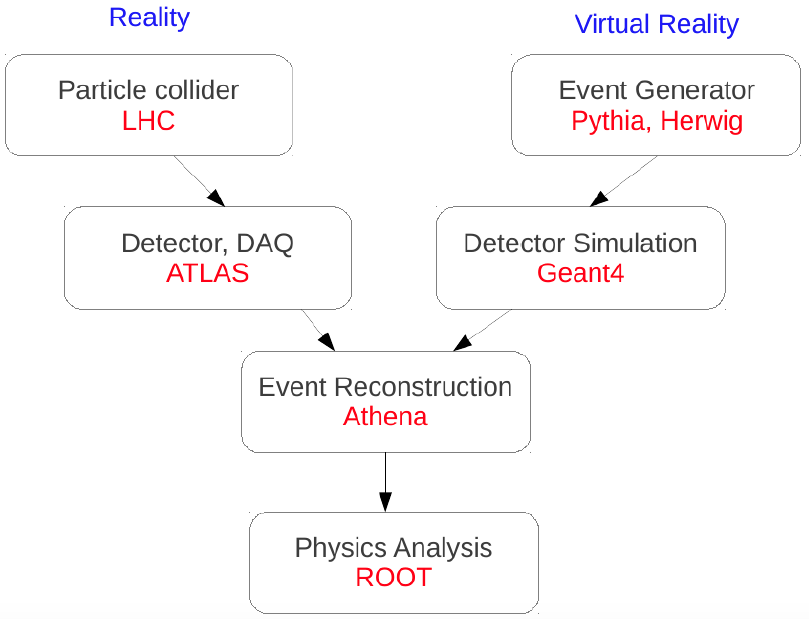
\includegraphics[scale=0.5]{figures/MC-diagram.png}
\caption{Work flow of standard analysis. \copyright John Morris.}
\label{fig:decays}
\end{figure}

The process of MC simulation from matrix elements to our observed decays before simulation of the detector can be described approximately with 8 steps.
=>Use google paint to create 8 step.
Each step can be performed in many different ways and this leads to theoretical modelling uncertainties. These uncertainties include generator,PDF,PS and hadronisation uncertainties. 
Generator uncertainties come from the limit on the order in which you calculate your matrix elements. PDF uncertainties come from the use of different parameterisations. At the LHC CTEQ, MSTW and NNPDF are used, each having a different result. PS uncertainties come from the divergencies that must be avoided in any QCD calculation. How this is dealt with depends on the generator. Two common example would come from the generators PYTHIA and HERWIG, which calculate the parton with the highest $p_T$ and angle respectively. Hadronisation occurs at very low energy scales in which perturbation theory is not valid. Therefore a suitable model is needed and two approaches are often used: the Lund string and Cluster models. Each model similarly to PS modelling will produce a different result, therefore this leads to further uncertainties in teh over all modelling. 
A general practice to determine the total uncertainty is by simply using different models for each calculation and taking the difference. 
At this stage known as the truth level the simulation has produced stable final state particles with all parent-daughter relations (i.e b-tagging from parton level) and 4 vector information. Now the interaction of the final state particle and the detector must be considered.       
GEANT4 is used to take the output 4-vectors of the truth level generator's and model the detector response. This is a very complex process and involves modelling all subdetectors of the ATLAS experiment. THis modelling can be done to different degrees of accuracy to save computation time and the final output matches the output of the ATLAS detector itself, i.e deposited charge on silcon device.   
